\rhead{Getting Started/Teleoperation}

\chapter{Getting Started/Teleoperation}
\label{sec:getting_started}

\begin{figure}[!h]
\centering
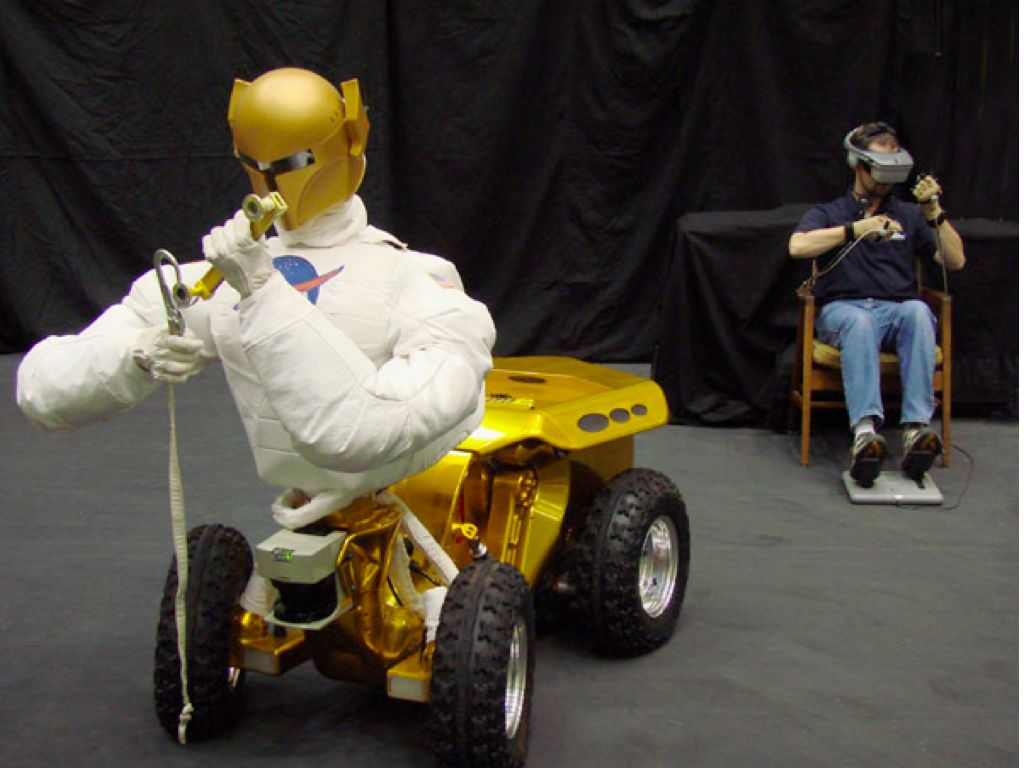
\includegraphics[width=1.0\columnwidth]{figures/2_teleop.jpg}
\end{figure}

\newpage

\begin{wrapfigure}{l}{0.55\columnwidth}
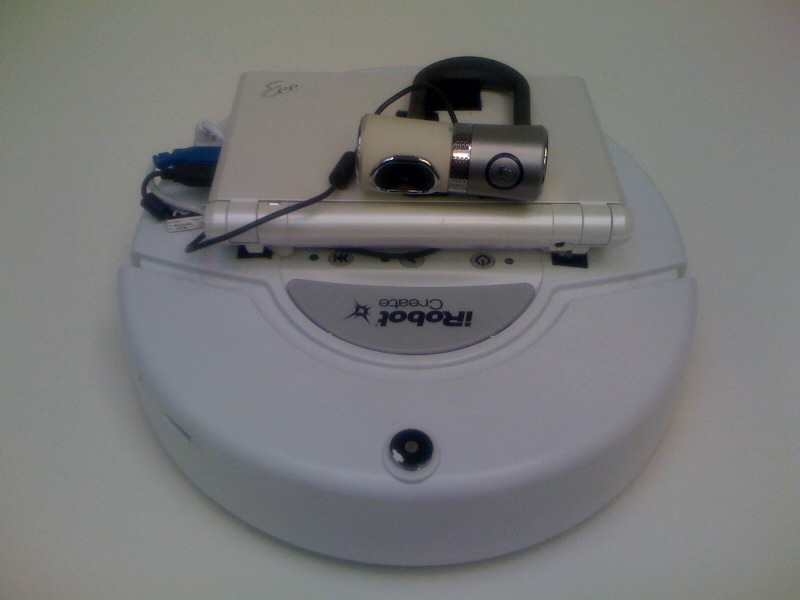
\includegraphics[width=0.5\columnwidth]{figures/2_teaser.jpg}
\end{wrapfigure}

In this chapter, we walk through the basic steps for assembling and remotely controlling a low-cost mobile robot, which we call the ``SmURV'', from ``commercial off-the-shelf'' (COTS) components.  At the completion of this chapter, you will have an assembled SmURV robot platform built with solderless commodity components. You will be able to remote control, or teleoperate, a mobile robot using one of two middleware packages we introduce in the chapter.  Instructions for hardware assembly and software installation are specified step-by-step. This chapter refers to \href{http://robotics.cs.brown.edu/projects/smurv}{The SmURV Robotics Platform}, which uses a previous version of the robot platform, and an updated version, \href{http://robotics.cs.brown.edu/projects/player\_icreate}{Setting up Player 2.1.1: Asus EeePC and iCreate Robot}. Please note, all the technology, instructions and hardware costs are as of Spring 2010.

The primary purpose of the SmURV  ({\bf Sm}all {\bf U}niversal {\bf R}obotics {\bf V}ehicle) is to be a robot platform that emphasizes the computational aspects of robotics without requiring engineering expertise or low-level hardware hacking.  That is, no soldering or low-level assembly programming is necessary to build a SmURV.  However, we do assume the reader has user-level knowledge of Unix (e.g., Ubuntu Linux, OS X) and super-user abilities to install software packages, etc.

The SmURV platform, as seen on the previous page, is based on the iRobot Create mobile base with a sub-notebook computer, such as the Asus EEE PC, and a webcam-style camera.  All of the hardware components for the SmURV can be readily purchased from online or brick-and-mortar stores, such as Target.  The computer typically runs some distribution of Linux (Ubuntu in our case) with a robot middleware package to mediate communication between a client application and the the Create/USB camera hardware.  We describe how to install robot middleware packages for Player and the Robot Operating System (ROS), although you will only need one.  Robot middleware is discussed in detail in Chapter \ref{sec:robot_middleware}.

At the end of this chapter you will be able to:
\begin{itemize}
\item Assemble a low-cost mobile robot using COTS components.
\item Install all the necessary software for running a robot client.
\item Teleoperate a mobile robot.
\end{itemize}

\section{Hardware Components}

\subsection{iRobot Create}

\begin{wrapfigure}[12]{r}{0.35\columnwidth}
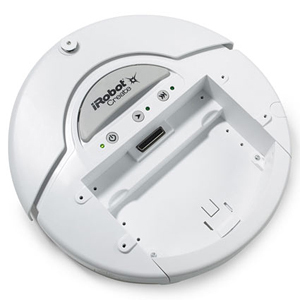
\includegraphics[width=0.3\columnwidth]{figures/2_create_base.jpg}
\end{wrapfigure}

The \href{http://store.irobot.com/shop/index.jsp?categoryId=3311368}{iRobot Create}, produced by \href{http://www.irobot.com/}{iRobot}, is used as the basic robot unit.  It is a mobile robot that is similar to the iRobot Roomba, except it does not contain a vacuum and is instead designed for robotics development.  The Create is equipped with a serial port; the \href{http://www.irobot.com/filelibrary/create/Create_Open_Interface_v6.pdf}{Open Interface Specification} (OIS) for the Create explains what commands can be sent to the Create over the serial port in order to read sensor data and send motor commands to the robot.  However, we do not 
teach students how to write programs by sending low level commands to the robot. Instead we utilize robot middleware (as explained in Chapter \ref{sec:robot_middleware}), as a hardware/software abstraction for transparency and portability.

\subsection{Accessories for the iRobot Create}
\begin{itemize}
\item \href{http://store.irobot.com/product/index.jsp?productId=2586254}{Serial Cable} that is packaged with the Create.

\item Serial to USB adapter cord.  CS148 uses FTDI US232R-10 ``evaluation cables'' which can be ordered from \href{www.digikey.com}{DigiKey} for roughly USD \$20.  Note: this cord needs to be of sufficient quality; cheaper adapters will overheat and cause problems.

\item (recommended) Rechargeable Advanced Power System (APS) Battery.

\item (optional) iRobot \href{http://store.irobot.com/product/index.jsp?productId=2731666&cp=2804606.3335976&ab=CMS_IRBT_CreateSuperCat_CreateAcc_111309&parentPage=family}{Virtual Wall} which creates an invisible barrier that the Create will not cross by emitting infrared signals that the Create detects with its IR receiver. 

\item (optional) Self Charging \href{http://store.irobot.com/product/index.jsp?productId=2598729&cp=2804606.3335976&ab=CMS_IRBT_CreateSuperCat_CreateAcc_111309&parentPage=family}{Home Base} which enables the Create to automatically charge its iRobot rechargeable battery.
\end{itemize}

\begin{figure*}
\centerline{
\mbox{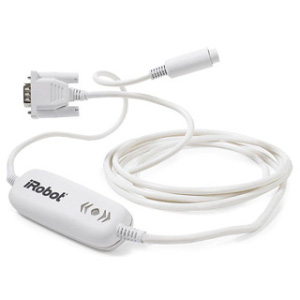
\includegraphics[width=1.50in]{figures/2_serial_cable.jpg}}
\mbox{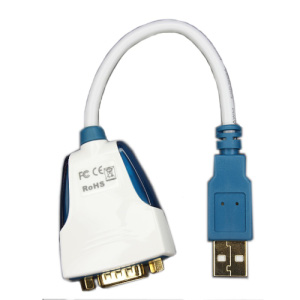
\includegraphics[width=1.50in]{figures/2_serialusb_cord.jpg}}
\mbox{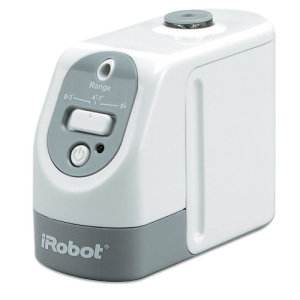
\includegraphics[width=1.50in]{figures/2_irwall.jpg}}
\mbox{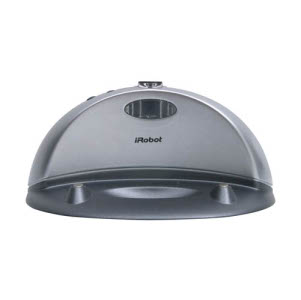
\includegraphics[width=1.50in]{figures/2_homebase.jpg}}
}
\caption{iRobot accessories include a serial cable, a serial to USB adapter, a virtual wall and a self charging home base.}
\end{figure*}

\subsection{Asus EeePC subnotebook}

\begin{wrapfigure}[8]{hr}{0.25\columnwidth}
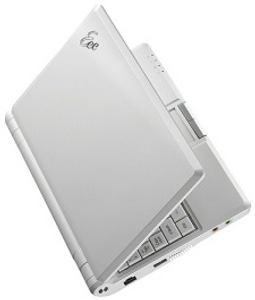
\includegraphics[width=0.2\columnwidth]{figures/2_eeepc.jpg}
\end{wrapfigure}

The \href{eeepc.asus.com/}{Asus EeePC} subnotebook is the computational brain for this robot platform.  The EeePC communicates with the Create base through a USB-Serial connection. Programs running on the EeePC will control the robot's actuators and receive sensory information. Thus the programmer does not have to worry about sending low level commands to the Create's serial port.  We recommend the \href{http://www.asus.com/index.aspx}{7'' EeePC} model since larger EeePCs will stick out over the Create base.

\subsection{USB Camera}

\begin{wrapfigure}[6]{hr}{0.25\columnwidth}
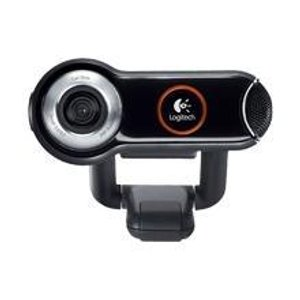
\includegraphics[width=0.2\columnwidth]{figures/2_webcam.jpg}
\end{wrapfigure}

Just having the bump, cliff and IR sensors built into the Create is not necessarily a lot of fun. Adding a camera to the robot however is! You can either go with a cheap USB Webcam or a more expensive Firewire camera if having uncompressed high quality images is a requirement. CS148 previously utilized a Unibrain Fire-I camera. However with our newest platform we recommend a USB webcam, preferably a newer, Video4Linux2 (V4L2) version.

\subsection{Assembling the Robot Platform}
\label{sec:assembling_the_robot_platform}

\begin{enumerate}
\item Connect the Create's serial cable to the USB to serial adapter. Connect this to the Create and the EeePC, as seen in Figure \ref{fig:2_cable_setup}, left image.
\item Connect the USB webcam to the EeePC.
\item Tuck the cords into the Create and set the EeePC on top. The assembled Create platform is seen in Figure \ref{fig:2_cable_setup}, right image.
\item Optionally, add Velcro tape to secure the EeePC to the top of the Create and to secure the camera to the EeePC.
\end{enumerate}

\begin{figure}[!h]
\centerline{
\mbox{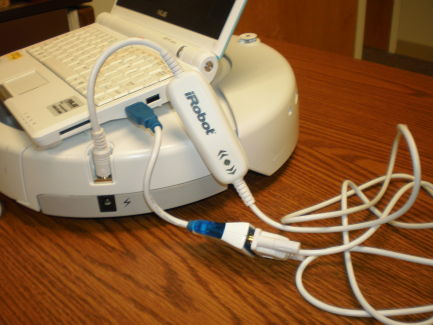
\includegraphics[width=3.00in]{figures/2_cable_setup.jpg}}
\mbox{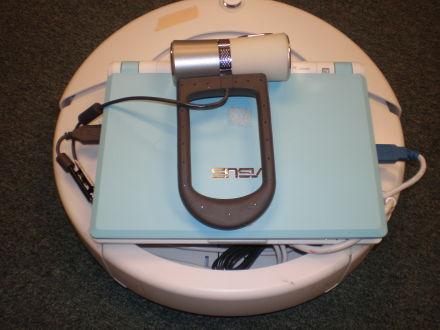
\includegraphics[width=3.00in]{figures/2_cable_store.jpg}}
}
\caption{Connected Create and EeePC; Assembled Create Robot Platform.}
\label{fig:2_cable_setup}
\end{figure}

\newpage

\subsection{Costs}

Costs are as of Spring 2010 and are specified in USD.

\begin{center}
    \begin{tabular}{ | p{3.0cm} | p{10cm} | l | l |}
    \hline
    \textbf{Part} & \textbf{Name} & \textbf{Cost} \\ \hline
    Robot (Basic) & \href{www.irobot.com}{iRobot Create Programmable Robot} & 129.99 \\ \hline
    Robot (Package) & \href{www.irobot.com}{iRobot Create Premium Development Package}; includes APS, 2 virtual walls, home base, remote and command module & 299.99 \\ \hline
    Subnotebook & \href{eeepc.asus.com}{Asus EeePC 7'' 2G Surf} & 240.00 \\ \hline
    USB Camera & \href{www.logitech.com}{Logitech Webcam Pro 9000} & 99.99 \\ \hline
    Serial to USB adapter & \href{www.digikey.com}{FTDI US232R-10 ``evaluation cables''} & 22.00 \\ \hline
    \end{tabular}
\end{center}

\section{Software Components}

\subsection{Operating System}
\label{sec:2_operating_system}

The EeePC comes with a GNU Linux OS, however we recommend installing \href{http://www.geteasypeasy.com/}{Easy Peasy (formerly Ubuntu-Eee)}, which is a custom version of Ubuntu designed especially for the EeePC.  The EeePC comes with a version of Xandros Linux which has Asus-modified libraries that are incompatible with the Player middleware system (see Section \ref{sec:player213}), thus it is recommended to simply install a more standard OS.  Easy Peasy was chosen because it is one of the more supported custom Eee Linux distributions available and it is one of the few that fits on the EeePC 2G Surf model. Note: other distributions are available and outlined on \href{http://wiki.eeeuser.com/#installing\_operating\_systems}{Installing Operating Systems}, but the rest of the instructions are assuming an Easy Peasy installation.

\subsubsection{\href{http://robotics.cs.brown.edu/projects/player_icreate/u_install.html}{Install Easy Peasy}}

\begin{enumerate}

\item You will need:
\begin{itemize}
\item Another computer to download Easy Peasy on and to run UNetbootin (Universal Netboot Installer) for creating a bootable USB flash drive. This computer must be either Windows or Ubuntu/Linux. If using Linux, you will need administrative rights to install the UNetbootin application.
\item An empty USB stick (of 1GB or more, formatted to FAT32) to do the initial Ubuntu boot and installation. 

\end{itemize}

\item From the secondary computer, go to the \href{http://www.geteasypeasy.com/}{Easy Peasy download site} and click on ``Download''.

\item Select the ``Download" link to download Easy Peasy and choose ``Save File" (Figure \ref{fig:easy_peasy}).
\begin{figure}[!h]
\centering
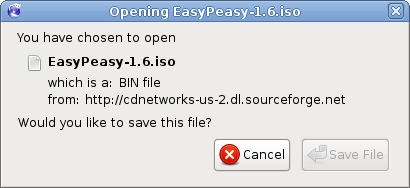
\includegraphics[width=0.5\textwidth]{figures/2_download_easypeasy2.png}
\caption{Easy Peasy download screenshot.}
\label{fig:easy_peasy}
\end{figure}


\item Download UNetbootin, a helper application used to move Easy Peasy to a USB stick. On the \href{http://unetbootin.sourceforge.net/}{UNetbootin site}, select either ``Download (for Windows)'' or ``Download (for Linux)'' depending on your operating system. Select ``Save File" (Figure \ref{fig:unetboot_download}). This step of creating a bootable drive is necessary since the EeePC does not have a CD-ROM drive.

\begin{figure}[!h]
\centering
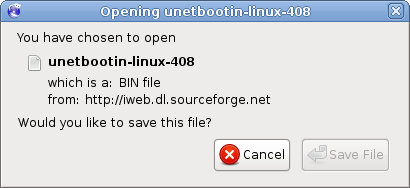
\includegraphics[width=0.5\textwidth]{figures/2_download_unetbootin.png}
\caption{UNetbootin download screenshot.}
\label{fig:unetboot_download}
\end{figure}

\item Make sure the USB stick is formatted to FAT32, otherwise the installation of Easy Peasy on the EeePC will hang and be unsuccessful. Note: formatting the stick will cause all data to be lost.

\begin{itemize}
\item To format the USB stick in Windows, insert the stick and right click on the USB icon. Press ``Format" in the menu. Select ``FAT32" in the File system drop-down list and press ``Start" (Figure \ref{fig:2_fat32}).

\begin{figure}[!h]
\centering
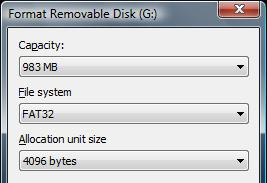
\includegraphics[width=0.35\textwidth]{figures/2_fat32.jpg}
\caption{Formatting to FAT32 in Windows.}
\label{fig:2_fat32}
\end{figure}

\item To format the USB stick in Linux, root permissions are necessary. Insert the USB stick.

\begin{enumerate}

\item Determine if the USB is already formatted to FAT32. Run: \\
\texttt{sudo fdisk -l}

\begin{figure}[!h]
\centering
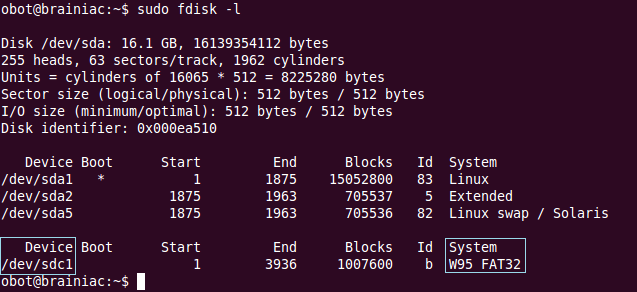
\includegraphics[width=0.66\textwidth]{figures/2_fat32_ok.png}
\caption{List USB device and current formatting.}
\label{fig:2_fat32_ok}
\end{figure}

If FAT32 is listed under ``System" (Figure \ref{fig:2_fat32_ok}), you do not need to reformat. If anything else is listed, continue.

\item Determine which device (sda, sdb, sdc, etc) Linux assigned the USB drive to. Running the above \texttt{fdisk} command prints this information under ``Device" (Figure \ref{fig:2_fat32_ok}). In our case the device assignment is to ``/dev/sdc1".\label{sec:format_usb_stick}

\item Run \href{http://linux.die.net/man/8/fdisk}{fdisk}, a partition table manipulator: \\
\texttt{sudo fdisk /dev/sdX}\\
\texttt{sdX} should be the name of the device as determined in the previous step.

\item Enter ``d" to delete all existing partitions.

\item Enter ``n" to create a new partition.\\ 
Enter ``p" for the command action.\\
Enter ``1" for the partition number.\\
Hit Enter twice to keep default settings.

\item Enter ``t" to impose the partition's system type as FAT32.\\
Enter ``b" as the partition type hex code, which is the id for type FAT32.

\item Enter ``w" to save changes and write the partition table to the USB stick.

\begin{figure}[!h]
\centering
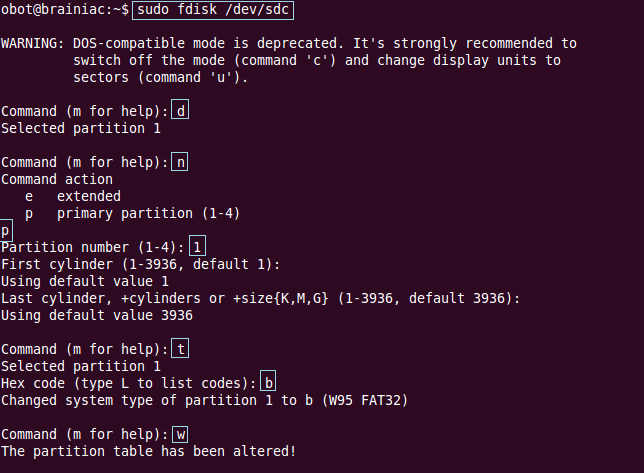
\includegraphics[width=0.66\textwidth]{figures/2_create_partition.png}
\caption{Steps (c) - (g).}
\end{figure}

\item Unmount the device: \texttt{sudo umount /dev/sdX1}

\item Format the drive to FAT32:\\
\texttt{sudo mkfs.vfat -F 32 /dev/sdX1}\\
This step is necessary in order to format the newly created partition.

\begin{figure}[!h]
\centering
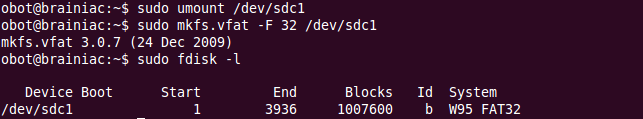
\includegraphics[width=0.66\textwidth]{figures/2_format_fat32.png}
\caption{Steps (h) - (i).}
\end{figure}

\item Unplug and insert the USB stick into the computer again.

\end{enumerate}

\end{itemize}

\item Install UNetbootin:\footnote{The following are the same instructions as under ``Installation \& Screenshots" on the \href{http://unetbootin.sourceforge.net/}{Unetbootin site}}
\begin{itemize}
\item Run the UNetbootin executable.

\begin{itemize}
\item If using Windows, click on the UNetbootin file to launch the application (Figure \ref{fig:unetboot_windows}).
\begin{figure}[!h]
\centering
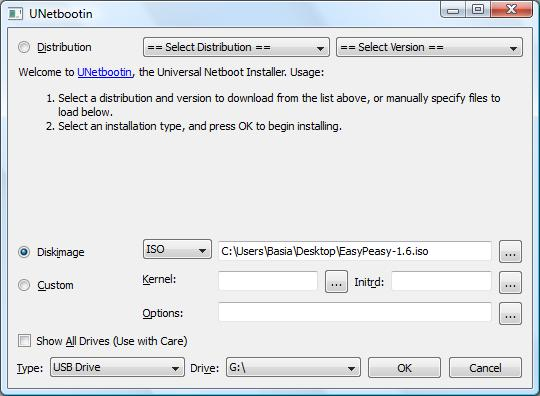
\includegraphics[width=0.85\textwidth]{figures/2_unet_windows.jpg}
\caption{UNetbootin installation prompt for Windows.}
\label{fig:unetboot_windows}
\end{figure}

\item If using Linux:\\
\begin{itemize}
\item Install Unetbootin dependencies:\\
\texttt{sudo aptitude install mtools p7zip-full}
\item Make the file executable:\\
\texttt{chmod +x unetbootin-linux-*}
\item Run the application (Figure \ref{fig:unetboot_linux}):\\
\texttt{sudo ./unetbootin-linux-*}
\end{itemize}
\begin{figure}[!h]
\centering
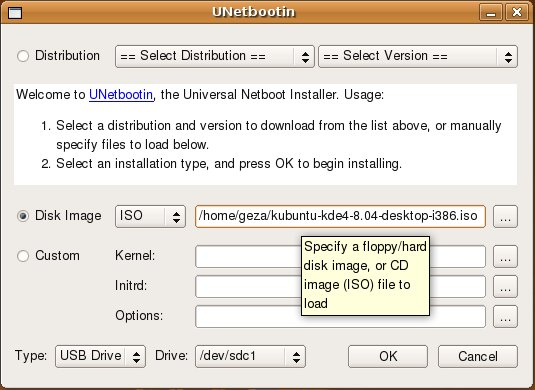
\includegraphics[width=0.85\textwidth]{figures/2_unet_linux.jpg}
\caption{UNetbootin installation prompt for Linux.}
\label{fig:unetboot_linux}
\end{figure}

\end{itemize}

\item Select Distribution/Select Version may be ignored. The Disk Image format should be ``ISO"; enter ``EasyPeasy-*.iso" (the downloaded Easy Peasy file) as the Disk Image. This specifies which file to create the bootable drive from. Finally select ``USB Drive" as the Type and specify the target Drive. Press ``OK".
\begin{itemize}
\item If using Windows, refer to Figure \ref{fig:unetboot_windows}.
\item If using Linux, refer to Figure \ref{fig:unetboot_linux}. By default, the correct USB drive should be automatically selected. To be certain, the instructions to find the name of the USB drive are outlined in step \ref{sec:format_usb_stick}.
\end{itemize}

\item After installation is complete (prompted by the screenshot in Figure \ref{fig:unetboot_install_complete}), do not reboot and instead select ``Exit" (unless you are installing Easy Peasy on the same EeePC from which you create the bootable USB drive). Unmount the disk. Easy Peasy is now installed on the USB stick.
\begin{figure}[!h]
\centering
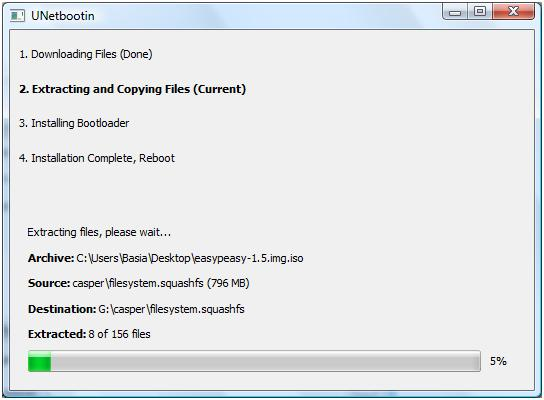
\includegraphics[width=0.85\textwidth]{figures/2_unet_windows1.jpg}
\caption{UNetbootin installation screenshot.}
\label{fig:unetboot_install}
\end{figure}

\begin{figure}[!h]
\centering
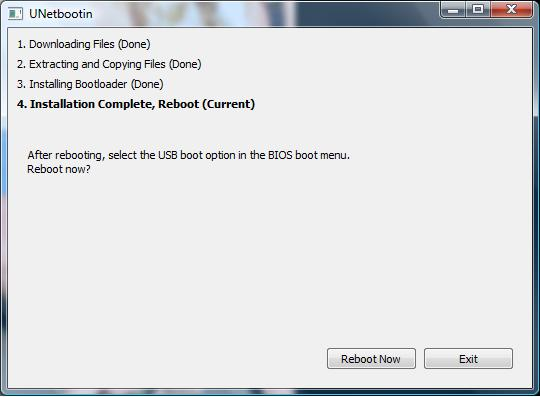
\includegraphics[width=0.85\textwidth]{figures/2_installation_complete.jpg}
\caption{UNetbootin installation complete screenshot.}
\label{fig:unetboot_install_complete}
\end{figure}

\end{itemize}

\item Insert the USB stick into the EeePC\footnote{It is suggested to use the USB port on the left side of the EeePC; some EeePC's seem unable to boot from the USB ports on the right side.}

\item (Re)start the EeePC. Press ESC a few times while the Asus boot screen is displayed.

% press F2 quickly while the EeePC is starting; this will take you to the BIOS Setup Screen. In the ``Boot" tab, select the ``Boot Device Priority" subscreen by pressing Enter. Make sure the USB drive is selected as the Boot option.

\item Select the USB drive from the list of bootable devices in the boot menu.

\item Select ``Default" from the UNetbootin menu.

\item Install Easy Peasy by selecting the ``Install EasyPeasy 1.*" icon, which should be in the Desktop folder.

\item You will be prompted for your language preference, time zone, etc. Follow all the installation instructions.

\item If your EeePC is the 2G Surf model, be aware that there is only 2GB of hard drive and the OS takes up 1.8GB when you install. Tips to prevent wasted time reinstalling:
\begin{itemize}
\item Choose ``No Localization'' on the first install screen.
\item Do a manual install, with an ext2 format and no swap drive.
\item Once installed, the 2GB internal drive will be nearly full. To free more than 300mB, uninstall Open Office, Skype and other unnecessary applications using the following command:\\
\texttt{sudo apt-get remove <package\_name>}\\
where \texttt{<package\_name>} is any package, such as \texttt{openoffice.org*}. Note, to list all installed packages: \texttt{dpkg --list}\\
\end{itemize}

\item (Optional) Enable the Regular Desktop mode instead of the Netbook Interface mode by following these \href{http://wiki.geteasypeasy.com/How_to_use_Regular_Desktop_mode_instead_of_the_Netbook_Interface_mode}{instructions}.

\item Connect the EeePC to the internet (necessary for the next step).

\item \label{sec:2_enable_repos}Enable all of the repositories in the \texttt{/etc/apt/sources.list} file. Ubuntu uses \href{http://www.debian.org/doc/manuals/apt-howto/}{APT} for package management; \texttt{/etc/apt/sources.list} contains a list of sources from which software repositories can be obtained.
\begin{itemize}
\item Backup the configuration file: \\
\texttt{sudo cp /etc/apt/sources.list /etc/apt/sources.list.backup}
\item Open the file for editing: \texttt{sudo nano /etc/apt/sources.list}
\item Enable all software repositories by uncommenting any commented-out apt repository lines (lines which begin with either ``deb" or ``deb-src"). The following are two apt lines:\\
\texttt{deb http://us.archive.ubuntu.com/ubuntu/ lucid main restricted}\\
\texttt{deb-src http://us.archive.ubuntu.com/ubuntu/ lucid main restricted}
\item Obtain the updated package lists from the newly enabled repositories:\\
\texttt{sudo apt-get update}\\
If you get the error ``Failed to fetch...", make sure the EeePC is connected to the Internet!
\item If you are outside the US and receive a ``Failed to fetch..." error, try changing all references from ``http://us.archive.ubuntu.com" to ``http://archive.ubuntu.com" in the \texttt{sources.list} file.
\end{itemize}

% \item Install software updates using the Update Manager, which can be found under ``System" $\rightarrow$ ``Administration" $\rightarrow$ ``Update Manager". DO NOT let the Update Manager remove any Ubuntu Eee specific packages (it may try).

\item Install others software packages that will be utilized: \\
\texttt{sudo apt-get install cmake subversion wget python g++}\\
If using only Player, none of these are essential for teleoperation, but cmake and subversion are at least highly recommended. If using ROS, all four of these are necessary.

\end{enumerate}


\subsection{Player 2.1.3}
\label{sec:player213}

\subsubsection{Install Player 2.1.3}
After installing Easy Peasy, the EeePC is now ready to \href{http://playerstage.sourceforge.net/doc/Player-2.1.0/player/install.html}{install Player}.

\begin{enumerate}
\item Download \texttt{player-2.1.3.tar.gz} source tarball from \href{http://sourceforge.net/projects/playerstage/files/}{Player Sourceforge Site}.

\begin{figure}[!h]
\centering
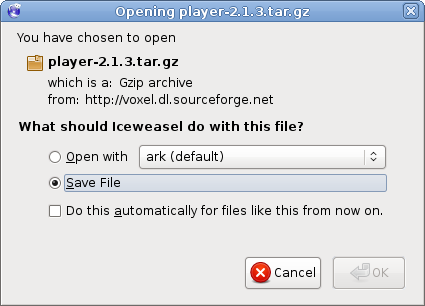
\includegraphics[width=0.5\textwidth]{figures/2_opening_player.png}
\caption{Download Player 2.1.3 screenshot.}
\label{fig:open_player}
\end{figure}

\item Uncompress and expand the downloaded file: \texttt{tar xzvf player-2.1.3.tar.gz}

\item Install additional libraries: \texttt{sudo apt-get install <library\_name>}\\
Replace \texttt{<library\_name>} with each of the following libraries: \\
libgdk-pixbuf2, libgtk2.0-dev, libjpeg62-dev.\\  
\texttt{apt-get} should have all of these libraries if every repository in \texttt{/etc/apt/sources.list} has been enabled (refer to step \ref{sec:2_enable_repos} of Section \ref{sec:2_operating_system}).
\begin{itemize}
\item If running \texttt{apt-get} gives the error: ``Couldn't find package libgdk-pixbuf2":
\begin{itemize} 
\item Add the following lines to the \texttt{/etc/apt/sources.list} file:\\
\texttt{deb http://us.archive.ubuntu.com/ubuntu/ jaunty universe}\\
\texttt{deb-src http://us.archive.ubuntu.com/ubuntu/ jaunty universe}\\
\texttt{deb http://us.archive.ubuntu.com/ubuntu/ jaunty-updates universe}\\
\texttt{deb-src http://us.archive.ubuntu.com/ubuntu/ jaunty-updates universe}\\
\item Run: \texttt{sudo apt-get update}\\
\end{itemize}

\item If you are using a fireware camera and not a USB webcam, you should also \texttt{apt-get install} the following libraries: \\ libraw1394-dev, libavc1394, libdc1394-13, libdc1394-13-dev.
\end{itemize}

\item Change to the Player source directory: \texttt{cd player-2.1.3}

\item Configure Player: \texttt{./configure}\\
Note: Player will install without throwing any errors regardless if libraries are missing. If the above mentioned libraries were not installed, Player will still install but either Player or accessing camera data may not work.

\item To enable Player to have more functionality beyond using the Create, the sensor drivers, a USB or camera, the blobfinder proxy, and playercam/playerjoy, it may be necessary to install more libraries. The libraries needed are located in the \texttt{player-2.1.3/config.log} file, which was created by configure. \texttt{config.log} is a huge file that contains all the messages created by configure, including missing packages, library dependencies and a list of what Player has and has not installed.

\item Compile Player: \texttt{make}.

\item Install Player: \texttt{sudo make install}.

\item Restart the EeePC.

\item Reopen the terminal and run Player: \texttt{player} 
\begin{itemize}
\item The output should be similar to Figure \ref{fig:player_output}.
\label{sec:player_output}

\begin{figure}[!h]
\centering
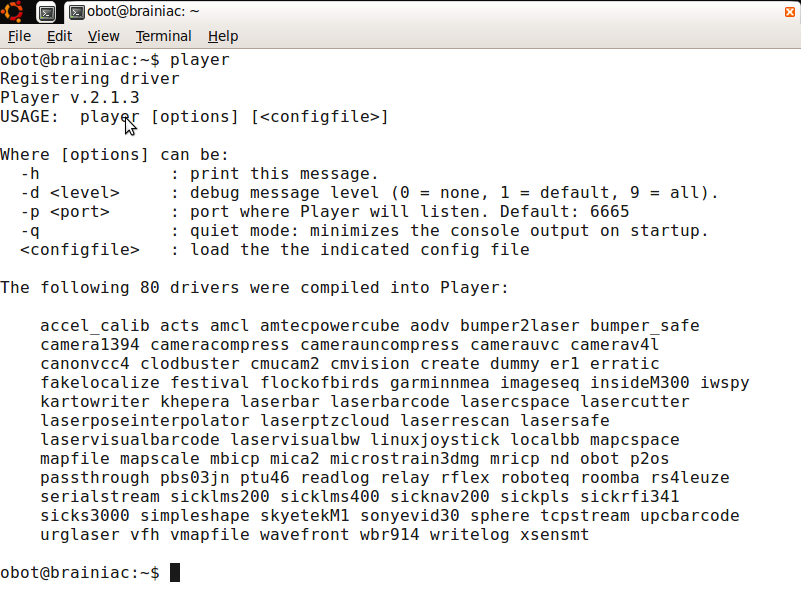
\includegraphics[width=0.85\textwidth]{figures/2_player_output.png}
\caption{Output from starting Player (Step \ref{sec:player_output} in ``Install Player 2.1.3'' instructions).}
\label{fig:player_output}
\end{figure}

\item If the following message is displayed:\\

player: error while loading shared libraries: libplayerdrivers.so.2.2: cannot open shared object file: No such file or directory\\

Run \texttt{ldconfig} to fix the error. Player sometimes does not link its libraries completely when installing.

\item If the ``Registering driver'' message outputs from Player, installation is successful and the EeePC is now ready to be hooked up to the  robot.
\end{itemize}

\end{enumerate}

\subsubsection{Run and Test Player on the Create}

To test the robot's vision and to teleoperate the Create, in this section we will be running two Player utilities that are included with the Player distribution: \href{http://playerstage.sourceforge.net/doc/Player-cvs/player/group__util__playercam.html}{playercam} and \href{http://playerstage.sourceforge.net/doc/Player-cvs/player/group__util__playerjoy.html}{playerjoy}. playercam is a GUI client that visualizes the images captured by the webcamera. playerjoy provides mobile control of the robot. The playerjoy client uses input from the keyboard to drive the robot around; only a forward and rotate speed can be manipulated on the Create.

\begin{enumerate}

\item You will need:
\begin{itemize}
\item The assembled Create Robot Platform.
\item The EeePC installed and working with Player.
\item Ideally (but not necessary to test) a wireless network and another computer with Player installed.
\end{itemize}

\item Create a configuration file, which is required by the Player server to tell Player what robot systems to load drivers for. Configuration files are text files that have a \texttt{.cfg} extension. Below is \texttt{create.cfg}, a basic configuration file for the Create with position and bumper proxies specified along with camera/blobfinder drivers. The following configuration file assumes the robot is attached to the ``/dev/ttyUSB0" port. If the robot is actually attached to a different port, reflect this change in the configuration file.

\begin{verbatim}
driver
(
        name "create"
        provides ["position2d:0" "bumper:0" "power:0" "ir:0"]
        port "/dev/ttyUSB0"
)

driver
(
        name "camerauvc"
        provides ["camera:0"]
)

driver
(
        name "cmvision"
        provides ["blobfinder:0"]
        requires ["camera:0"]
        colorfile "colors.txt"
)
\end{verbatim}

You will pass the name of this configuration file as a command line argument when starting the Player server. Please refer to Section \ref{sec:player_quickstart} for an explanation of Player configuration files and the specific format.

Note: if your EeePC has a built-in webcam, you will have to specify the external camera in the config file.
\begin{itemize}
\item Under the line:   provides [``camera:0'']   add the line:   port ``/dev/video0''.
\item Check whether your external cam is video0 or video1 by listing the contents of the \texttt{/dev} directory with the camera plugged in and unplug the camera to see which listing disappears.
\end{itemize}

\item Create a color calibration file for the blobfinder proxy. This color file is specified as \texttt{colors.txt} in the above configuration file, thus this file must reside in the same directory as \texttt{create.cfg}. Below is a generic uncalibrated color file.

\begin{verbatim}
[Colors]
(255,  0,  0) 0.000000 10 Red
(  0,255,  0) 0.000000 10 Green
(  0,  0,255) 0.000000 10 Blue

[Thresholds]
( 25:164, 80:120,150:240)
( 20:220, 50:120, 40:115)
( 15:190,145:255, 40:120)
\end{verbatim}

The following is a sample color file that has been calibrated for four different colors.

\begin{verbatim}
[Colors]
(255,  36,  0) 0.000000 10 Orange
(  0,255,  0) 0.000000 10 Green
(255,105, 180) 0.000000 10 Pink
(255, 255,0) 0.000000 10 Yellow

[Thresholds]
( 100:135, 101:115, 170:214)
( 20:220, 50:120, 40:115)
( 99:132, 123:131, 168:207)
( 124:174, 90:105, 137:148)
\end{verbatim}
Note, in a color calibration file, there must be a line space in between the Colors and the Thresholds sections. Details on what the numbers in the color file represent and how to calibrate for colors will be explained in Chapter \ref{sec:object_seeking}.

\item Put a charged battery in the Create base, turn on both the Create and the EeePC. The Led lights on the Create will blink and eventually turn off; even if the lights stop blinking the Create may still be turned on.

\item Start the Player server. Open a terminal and \texttt{cd} to the directory where your configuration file is and type: \texttt{player create.cfg}\\
\label{sec:run_player_server_output}If all is successful you should get a similar message displayed in Figure \ref{fig:player_on}.

\begin{figure}[!h]
\centering
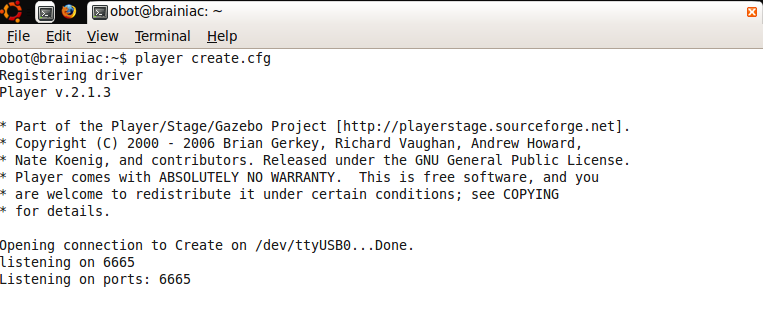
\includegraphics[width=0.85\textwidth]{figures/2_player_on.png}
\caption{Output from running the Player server with a config file (Step \ref{sec:run_player_server_output} in ``Test and Run Player" instructions).}
\label{fig:player_on}
\end{figure}

The Player server is now running on your Create Robot.

\item Run playercam. In a second terminal on the EeePC, run: \texttt{playercam}\\
Running this command will open up a window on the screen with the camera's output, as seen in Figure \ref{fig:2_playercam}. If the EeePC is on a wireless network and you want to run playercam from another computer on the network, run:\\
\texttt{playercam -h <robot IP> -p 6665} \\
\texttt{<robot IP>} is the IP address of the EeePC. The port number could be different that \texttt{6665} if you have changed from the default. 

\begin{figure}[!h]
\centering
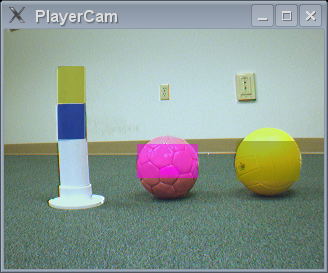
\includegraphics[width=0.5\textwidth]{figures/2_blobs.png}
\caption{Playercam output.}
\label{fig:2_playercam}
\end{figure}

If there are solid color rectangles over regions of the screen, the Player blobfinder works and is successfully detecting colors.

\item Run playerjoy to move the robot using keyboard commands. Preferably from a client computer on the network, run: \texttt{playerjoy <robot IP>:6665}. If running locally, just run: \texttt{playerjoy}. The terminal window output from running playerjoy is displayed in Figure \ref{fig:playerjoy}.
\begin{figure}[!h]
\centering
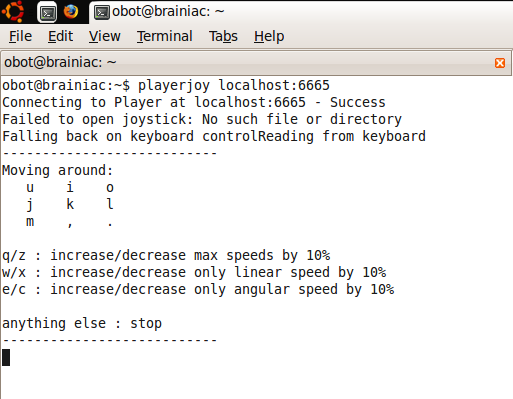
\includegraphics[width=0.6\textwidth]{figures/2_playerjoy.png}
\caption{Output from running playerjoy.}
\label{fig:playerjoy}
\end{figure}
 
Possible issues:
\begin{itemize}
\item If the robot does not move, make sure the Create base has not turned off and that the terminal with playerjoy running is selected/on top.
\item If the Create does turn off, both the player server and the client application (playerjoy or playercam) must be restarted.
\end{itemize}

\end{enumerate}


\subsection{ROS}
\label{sec:ros}

The \href{http://www.ros.org/wiki/ROS/Installation/Ubuntu/Deb}{ROS website} has installation instructions for Ubuntu that we will follow in addition to installing Brown's ROS packages. Brown University has a repository for ROS packages at \href{http://code.google.com/p/brown-ros-pkg/}{brown-ros-pkg}. Please check this site under the ``New Users" section for the latest instructions and updates on the software resources available.

\subsubsection{ROS Setup}

\begin{itemize} 

\item During the installation of Easy Peasy, make sure wget, Python, CMake and Subversion are all installed on the EeePC. If not, for any missing package needed:\\ 
\texttt{sudo apt-get install cmake subversion wget python}

\item Setup sources.list:\\
\texttt{sudo sh -c 'echo "deb http://code.ros.org/packages/ros/ubuntu karmic main" > /etc/apt/sources.list.d/ros-latest.list'}

\item Set up your keys:\\
\texttt{wget http://code.ros.org/packages/ros.key -O - | sudo apt-key add -}

\item Run: \texttt{sudo apt-get update}

\item Install: \texttt{sudo apt-get install ros-boxturtle-base}\\
Alternatively, for the latest release, run: \\
\texttt{sudo apt-get install ros-latest-base}

% \item Uninstall ros-specific packages???

\item Brown has a ROS install script available which retrieves versions of the ROS source, tested to be compatible with brown's packages, and automatically retrieves the latest brown packages. To retrieve the install script, on the EeePC run:\\
\texttt{wget http://brown-ros-pkg.googlecode.com/svn/tags/getros/getros.py}

\item Run the script to install: \texttt{python getros.py}

\item To setup the correct environment variables, from the ROS root directory run:\\ \texttt{source rosenv}\\
You must do this everytime you open up a new terminal.

\item Build the basic ROS packages with: \texttt{rosmake roslite} \\
Each brown-ros-pkg package can be build with appropriate calls to rosmake, such as: \texttt{rosmake cv\_capture}. Note, the \texttt{rosmake} command can be run from any directory within the ROS directory structure.

% sudo apt-get install python-yaml libapr1-dev libbz2-dev python-dev libaprutil1-dev python-numpy graphviz

%YAML
% If you receive a compile error: ``ImportError: No module named yaml", you need to install YAML.
% download from: http://pyyaml.org/wiki/PyYAML
% tar zxvf PyYAML-*.tar.gz
% cd PyYAML-*
% python setup.py instal

% LOG4CXX
% cd ~/ros/ros-deps 
% wget http://pr.willowgarage.com/downloads/apache-log4cxx-0.10.0-wg_patched.tar.gz
% tar xzf apache-log4cxx-0.10.0-wg_patched.tar.gz
% cd apache-log4cxx-0.10.0
% ./configure --prefix=/opt/ros
% make
% sudo make install 

% BOOST
% cd ~/ros/ros-deps
% wget --tries=10 http://pr.willowgarage.com/downloads/boost_1_37_0.tar.gz
% tar xzf boost_1_37_0.tar.gz
% cd boost_1_37_0
% ./configure --prefix=/opt/ros
% make
% sudo make install 

\end{itemize}

\subsubsection{Run and Test the Brown ROS Create Driver}

\begin{itemize}

\item The \href{http://code.google.com/p/brown-ros-pkg/wiki/irobot\_create\_2\_1}{Brown ROS Create Driver} is located in the ``ros-1.0.0/pkg/irobot\_create\_2\_1" directory. 


% PYTHON-SERIAL
% tar zxvf pyserial-*.tar.gz
% cd pyserial-*
% python setup.py install
 

\item \href{http://pyserial.sourceforge.net/}{python-serial} is the only external dependency of the driver and must be installed.
\begin{itemize}
\item Go to \href{http://sourceforge.net/projects/pyserial/files/}{pyserial} to download.
\item Unpack the archive and install the package: \\
\texttt{tar zxvf pyserial-*.tar.gz}\\
\texttt{cd pyserial-*}\\
\texttt{python setup.py install}
\end{itemize}

\item Build: \texttt{rosmake irobot\_create\_2\_1}

\item In its own terminal run: \texttt{roscore}\\
This command launches the ROS Master, which must be running for other ROS nodes to locate each other and communicate.

\item The ROS Create node assumes the robot is attached to ``/dev/ttyUSB0". If it is not, run: \texttt{rosparam set /brown/irobot\_create\_2\_1/port PORT}\\
PORT should be the port to which the robot is actually attached to.

\item Run the create driver: \texttt{rosrun irobot\_create\_2\_1 driver.py}\\
This command runs the Create driver from the Brown ROS package. The purpose of this node is to provide other nodes with basic sensor information (e.g. whether or not a bumper has been pressed), as well as to provide basic movement control to other nodes for the Create.

\item Teleoperate the Create using the ``teleop\_twist\_keyboard" package.
\begin{itemize}
\item Compile: \texttt{rosmake teleop\_twist\_keyboard}
\item Run: \texttt{rosrun teleop\_twist\_keyboard teleop\_twist\_keyboard.py}
This teleoperates the robot using keyboard commands (Figure \ref{fig:2_teleop_twist}).
\end{itemize}

\begin{figure}[!h]
\centering
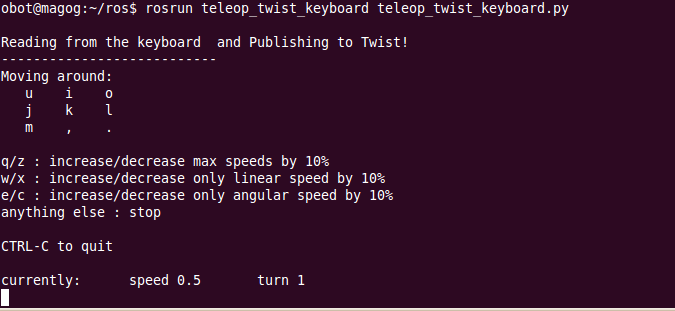
\includegraphics[width=0.8\textwidth]{figures/2_teleop_twist.png}
\caption{Teleoperating the Create using ROS}
\label{fig:2_teleop_twist}
\end{figure}


\end{itemize}

\newpage
